\documentclass[conference]{IEEEtran}
\IEEEoverridecommandlockouts
% The preceding line is only needed to identify funding in the first footnote. If that is unneeded, please comment it out.
\usepackage{cite}
\usepackage{amsmath,amssymb,amsfonts}
\usepackage{algorithmic}
\usepackage{graphicx}
\usepackage{textcomp}
\usepackage{xcolor}
\usepackage{flushend}
\usepackage{amsmath}
\usepackage{mathtools}
\usepackage[numbers]{natbib}
% \usepackage{tabularx}
\usepackage{tabularray}

\def\BibTeX{{\rm B\kern-.05em{\sc i\kern-.025em b}\kern-.08em
    T\kern-.1667em\lower.7ex\hbox{E}\kern-.125emX}}
\begin{document}

\title{An Empirical Study of Dependency Version Modification and API Breaking Changes}

\author{\IEEEauthorblockN{Mohammad Mahdi Abdollahpour}
\IEEEauthorblockA{\textit{Cheriton School of Computer Science} \\
\textit{University of Waterloo}\\
Waterloo, Canada\\
mohammadmahdi.abdollahpour@uwaterloo.ca}
}

\maketitle

\begin{abstract}
Among practitioners in the field of software engineering, it is well-known that change is the only constant of software development. Also, it is common for a project to use third-party libraries to implement at least parts of its desired functionalities. As a project evolves along with its dependencies, it becomes necessary or at least beneficiary for the developer of the project to change the version of its dependencies. However, API breaking changes can lead to necessary code changes, build failures, or unexpected behaviors; thus, it is vital to keep an eye on this aspect of software evolution both as the maintainer of a widely used library and as a client of third-party libraries. In this research, we conduct an empirical study to measure the prevalence of dependency version changes and API breaking changes in them. We present the results based on numerous Python projects along with two special case studies on widely used Python packages. We visualize the results using multiple graphs and tables to get an overview of the current status of the open-source software in the context of dependency and API changes.
\end{abstract}

\begin{IEEEkeywords}
Software Evolution, API Changes, Breaking Changes, Dependency Changes.
\end{IEEEkeywords}

\section{Introduction}
\textit{Motivation: }Many software systems use external code (libraries) as a code re-using technique to reduce the time of development for a particular feature. Software libraries also evolve over time. They might add or drop features or may change parts of the code behavior. Clients of these libraries use them via Application Programming Interfaces (APIs), which act as contracts between software systems. Some of the changes in software libraries could lead to changes in their APIs. And parts of those API changes can break backward compatibility, which is known as "API breaking changes." This type of breaking change can lead to several headaches for the downstream clients. The affected clients have several choices: they can choose not to upgrade the dependency or they can continue to use it. In the latter situation, either they have to risk breaking builds and unexpected behaviors (bugs) in their systems, or they have to invest development time in changing the codebase to conform to the new API. For this reason, many developers, tend to use mature and stable libraries. It allows them to have most of the features they want and at the same time, minimize the risk of dealing with API breaking changes in the future.

\textit{Research Goals: }In this study, we attempt to depict a high-level picture of the status quo in software development in terms of (I) the frequency of dependency version changes and (II) the amount of risk libraries pose to their clients. We conduct an empirical study over 188 Python projects to depict find out how frequently they change their dependencies. We continue our study further by analyzing each package version change to show the amount and frequency of version changes (upgrades and downgrades) throughout the whole history of 20 Python projects. To demonstrate how a project has to deal with API breaking change, we conduct a case study on one of the most frequently downgraded packages. Finally, we show, via a second case study, how a single package can pose a great deal of risk to a large number of projects, either directly or indirectly. We generate a dependency graph for one of the most widely used Python packages along with the number of API breaking changes (as a proxy to the amount of risk) of the target package and all of its dependencies.

\begin{figure*}[t!]
  \includegraphics[width=18cm,height=4cm]{figs/Untitled Diagram-Page-2.drawio.png}
  \caption{The overview of the study}
\end{figure*}

\section{Background \& Related Work}
There is a vast body of literature that focuses on the topic of API evolution and dependency changes. In a similar study to ours \cite{hist-brito}, \citeauthor{hist-brito} focus on a large corpus of Java projects to analyze API breaking change frequency and their evolution over time. They base their analysis on a tool \cite{apidiff} developed by a team of shared members. This study \cite{hist-brito} finds that 14.78\% of the API changes break compatibility with previous versions. They reach the conclusion that the frequency of breaking changes increases over time. We also reach a similar conclusion that the frequency of version changes increases over time in most projects. In another study \cite{jensjavabreak}, the authors find that there are more compatibility issues in libraries that use automated dependency resolution.

There are different reasons for developers to change the API of their libraries and there are different methods that convey their intent and help clients to adapt easier. In \cite{brito2016developers}, authors analyze the deprecation messages on API changes. Another paper \cite{brito2020you} tries to understand the motivations behind the API breaking changes. These two papers focus on Java libraries. In a similar study \cite{intent-api}, again on Java, \citeauthor{intent-api} perform a detailed analysis of the evolution of a production API according to its domain semantics and design intent.

\citeauthor{cox2019surviving} \cite{cox2019surviving} provides guidelines and recommendations for developers on dealing with API changes in software systems. \citeauthor{semdiff} \cite{semdiff} introduce a new tool that recommends replacements for a subset of API breaking changes (deleted methods). 



\section{Study Design}
% TODO brief summary 


\subsection{RQ1: How often do developers change their dependencies?}
\subsubsection{Identifying the projects that use \texttt{requirements.txt}}
We choose projects from TravisTorrent \cite{travistorrent}, a widely used dataset in this field. The dataset contains a significant amount of data related to build systems, which can be combined with our findings to derive new insights in the future.
We limit our analysis to Python projects as it is one of the most popular languages among engineers and researchers \cite{gholizadeh2022top}.
% Additionally, the lack of necessity for code compilation makes it easier for us to run static analysis on a larger number of projects.
In the first step, we clone 188\footnote{Two projects have private repositories as of writing this article.} projects using \texttt{LibGit2Sharp} library \cite{libgit2sharp}. Then, we filter out the projects that use dependency management methods other than \texttt{requirements.txt}. For this step, we used the \texttt{git} cli and its \texttt{log} search capability to search through all of the git histories of each project to capture any presence of \texttt{requirements.txt} files. 

\subsubsection{Extracting \texttt{requirements.txt} modifications}
We further analyze all of the commits modifying\footnote{We discard file deletion, addition, and renaming to simplify our analysis.} the \texttt{requirements.txt} file using \texttt{LibGit2Sharp} and only keep non-erroneous commits (i.e., having a parent commit, not facing formatting or file-system issues, etc) to make sure that we can compute a diff between two versions of the \texttt{requirements.txt} for each commit. From now on, we call these commits "requirement-changing commits" in this text. In total, we found 16385 requirement-changing commits.

\subsubsection{Extracting dependency version changes}
In the next step, we find the dependency version changes from the modified \texttt{requirements.txt} files. Detecting version changes is not a trivial task due to the way Python dependencies are specified in \texttt{requirements.txt}. For instance, one can define a package dependency like \texttt{numpy>=1.4.2} which means any version greater than or equal to \texttt{1.4.2} is acceptable for the dependency \texttt{numpy}. The developer can change this version specification in a commit to another specification like \texttt{numpy>=1.5.1,<1.7.4}. To determine if this change of specification is actually a downgrade or upgrade (or none) we need to find out the resolved version of the dependency at the time of each commit because it is mathematically not possible to compare two ranges in all cases. In the described example, the resolved version for the first specification could be \texttt{1.4.3} and for the second it could be \texttt{1.5.5} which is considered an upgrade. It could also be possible (based on the time of the change) that the first one would be resolved into \texttt{1.8.1} and the second into \texttt{1.7.3} which is a downgrade. 

Translation of each specification to a canonical resolved version involves two sub-tasks: For each requirement changing commit, we get the full release history of each package mentioned in the modified \texttt{requirements.txt} file from \texttt{pypi.org} (1). Then we filter the list of versions up until the time of commit based on the specification of that dependency (2). This is done by using the \texttt{packaging} library \cite{packaging}. Given a release version $V$ and a specification $S$, this library determines if $V$ satisfies $S$ based on the standards provided by \texttt{PEP 440}\cite{pep440}.

Furthermore, we categorize each specification change in each requirement modification into "upgrade," "downgrade," and "no change." 
Again, to compare each pair of the canonical versions we use \texttt{packaging} library which is based on \texttt{PEP 440}. 

The task of resolving all specifications in all requirement modifications involves thousands of web requests; hence we limit our study to the top 20 projects with less than 100 requirement modification commits. We find that, on average, each project has 35.5 version changes in all of its history, only about 6.8 of which are major version changes.

\subsection{RQ2: How much risk is involved in changing dependency versions?}

\subsubsection{Using \texttt{AexPy} to extract the API changes for each version change}
To answer the second research question, we use \texttt{AexPy} \cite{aexpy} to find the API changes. Given a package name $P$ and a version pair $V_{Before}, V_{After}$, \texttt{AexPy} generates a report that contains all of the API changes from $V_{Before}$ to $V_{After}$ in $P$. The report contains the type of each API change along with the count of non-breaking and breaking changes. It also categorizes breaking changes into three levels of severity. \texttt{AexPy} uses static analysis to calculate a identify the API changes based on a computed diff of the codebase in $V_{Before}$ and $V_{After}$. To compute this diff, it executes some preliminary steps to preprocess and extract the necessary information. In spite of the promising results in the original paper, we faced numerous failures in different stages of running \texttt{AexPy} in our studies. Moreover, unlike what is presented in the original paper \cite{aexpy}, it takes a relatively long time for \texttt{AexPy} to execute the analysis on each version change (more than 30 minutes in some cases). For these reasons, we approach the second research question by analyzing some case studies on a few selected projects.

\subsubsection{Case Study 1: Frequency of different types of API changes}
In the first case study, we want to see which type of API changes are more prevalent in a certain package. We use the \texttt{docker} image\footnote{https://hub.docker.com/r/stardustdl/aexpy} provided as the replication package of \texttt{AexPy} to execute the static analysis. We run this image on all version changes that have been found in the previous step for that package. Afterward, we parse and analyze the report file generated by the container. The results are presented in the next section.
\subsubsection{Case Study 2: API changes in the dependency graph}
In the second case study, we generate a dependency graph of a target package to get a sense of the impact in terms of API breaking changes in a bigger context (i.e., in relation to other packages). This graph (figure \ref{fig6}) depicts the dependencies and dependent packages of a chosen target package. We use the API provided by \texttt{libraries.io} to get the list of dependencies and dependent packages for the target package. For each dependency we find the count of API breaking changes by running \texttt{AexPy} on the latest version and the version from last year. The count of API breaking changes will be the weight of each edge from the target to each dependency. We also calculate the count of API breaking changes for one year period for the target package and put this value as the weight of inbound edges (i.e., the edges between dependents and target). Each edge resembles the amount of risk that has been posed by relying on a certain package. This graph could be extended further by adding more layers of dependencies and dependents. 

\section{Results}
In this section, we provide statistics and visualization as the results of the studies described in the last section. 

\subsection{RQ1: How often do developers change their dependencies?}

% \subsubsection{Modifications of the \texttt{requirements.txt} file}
% The frequency of dependency updates varies depending on the project and the developer. Some developers update their dependencies frequently to keep up with the latest features and bug fixes, while others may only update their dependencies when they encounter a bug or security issue. It is important to keep dependencies up-to-date to ensure that your project is secure and running smoothly. However, updating dependencies can also introduce new bugs and compatibility issues. 

In this part, our goal is to depict a high-level overview of the dependency changes among different projects.

\textbf{Approach.} First, we calculate the total number of the commits that change \texttt{requirements.txt} files in each project. 
Next, we calculate the average time of modification changes along with the rate of change over time for each project. To be more precise, for each commit time, we compute the exponential moving average of the duration between each two requirement-changing commits until that time. Then we plot the graph showing the change of the frequency (which is one over the computed average time) for each commit over the lifetime of the project (figure \ref{fig2}). We use the following formula to calculate the moving average:
\begin{multline*}
    EMA(C_N) =  (1 - \alpha) * EMA(C_{N-1}) + \\ \alpha * (CommitTime(C_N) - CommitTime(C_{N-1}))
\end{multline*}

Finally, we group the dependency version changes among the top 20 projects (as described in the previous section) by their name to identify which packages have the most version changes, upgrades, and downgrades.

\textbf{Results.} We can see the top five projects in table \ref{table1}. 

\begin{table}[h]
\centering
\caption{Top 5 projects with most requirement changing commits}
\begin{tblr}{
  width = \linewidth,
  colspec = {Q[538]Q[227]Q[150]},
  hlines,
  vlines,
}
\textbf{Project} & \textbf{\# Commits} & \textbf{\# Days}\\
GeoNode/geonode & 2848 & 4067\\
Kinto/kinto & 1493 & 3025\\
galaxyproject/galaxy & 977 & 2965\\
StackStorm/st2 & 738 & 3253\\
pydanny/cookiecutter-django & 510 & 3512
\end{tblr}
\label{table1}
\end{table}

From another perspective, we can see the histogram of the requirement changing commits in figure \ref{fig1}. 

\begin{figure}[h]
\centering
\begin{minipage}[h]{0.8\columnwidth}
  \includegraphics[width=\linewidth]{figs/newplot (6).png}
  \caption{Histogram of requirement changing commits per project. The histogram only shows projects with less than 100 commits for visualization purposes.}
  \label{fig1}
\end{minipage}\hfill
\end{figure}

We find that, on average, projects modify the \texttt{requirements.txt} file every 137 days. We also observe that most projects do this type of modification every 63 days (i.e., the median). More details are shown in figure \ref{fig2}.

\begin{figure}[h]
\centering
\begin{minipage}[h]{0.75\columnwidth}
  \includegraphics[width=\linewidth]{figs/newplot (7).png}
  \caption{Histogram of the average time between requirement changing commits per project. The histogram only shows projects with less than 200 commits for visualization purposes.}
  \label{fig2}
\end{minipage}\hfill
\end{figure}

We depict how \texttt{requirements.txt} modification rates change over time for several projects in figure \ref{fig3}.

\begin{figure}[h]
\begin{minipage}[h]{\columnwidth}
\centering
  \includegraphics[width=0.9\linewidth]{figs/newplot (1).png}
  \caption{Exponential moving average of the \texttt{requirements.txt} modification rate over time for five projects}
  \label{fig3}
\end{minipage}\hfill
\end{figure}

To see the modification rates from a broader point of view, we generated a 2D histogram (heatmap) of the requirement changing commits with a bin size of 2 months over the time of projects with more than 100 commits (figure \ref{fig4}). We filter out projects with fewer commits to prevent having a sizeable almost-blank area in the heatmap. 

\begin{figure}[h]
\begin{minipage}[h]{\columnwidth}
\centering
  \includegraphics[width=\linewidth]{figs/newplot (2).png}
  \caption{Heatmap of \texttt{requirements.txt} modification count over time for the projects having more than 100 commits}
  \label{fig4}
\end{minipage}\hfill
\end{figure}

By calculating the median, we find that most projects change package versions about 21 times (average: 35.5). This number is only 3 (average: 6.8) for major changes, and the rest are non-major (minor or patch) upgrades or downgrades. 

In table \ref{table2}, you can see the most changed dependencies among the top 20 projects. 

\begin{table}[h]
\centering
\caption{Packages with most version changes, upgrades, and downgrades}
\begin{tblr}{
  width = \linewidth,
  colspec = {Q[271]Q[30]Q[271]Q[30]Q[213]Q[28]},
  cell{1}{1} = {c=2}{0.301\linewidth},
  cell{1}{3} = {c=2}{0.301\linewidth},
  cell{1}{5} = {c=2}{0.241\linewidth},
  hlines,
  vlines,
}
\textbf{Change } &  & \textbf{Upgrade} &  & \textbf{Downgrade} & \\
\textbf{Package} & \textbf{\#} & \textbf{Package} & \textbf{\#} & \textbf{Package} & \textbf{\#}\\
certifi & 24 & certifi & 23 & pytest-xdist & 6\\
requests & 21 & requests & 20 & sphinx & 5\\
python-dateutil & 18 & python-dateutil & 17 & pillow & 4\\
pytest-xdist & 16 & lxml & 15 & releases & 4\\
lxml & 15 & gunicorn & 12 & numpydoc & 3
\end{tblr}
\label{table2}
\end{table}

\textbf{Analysis.} 
We see that different teams change the dependencies of their projects in different quantities and frequencies. However, most projects do not change their dependencies so often (only about every two months). We observe that teams have different patterns of modifying the dependencies, but overall, there has been a trend in recent years that most projects change their dependencies more frequently. Some packages are getting more updates, and others are getting the most downgrades. It is interesting to note that the most updated package in our study is \texttt{certifi} which is responsible for providing the most recent root certificates and is actually essential to be kept updated for security reasons \cite{certifi}.

\subsection{RQ2: How much risk is involved in changing dependency versions?}

\subsubsection{Case Study 1: Frequency of different types of API changes}

In this case, study, we analyze the API changes in \texttt{pytest-xdist}.

\textbf{Approach.} We choose the most downgraded package \texttt{pytest-xdist} from the previous part for further analysis in this case study. We want to see how many API changes and, more specifically, how many API breaking changes have occurred in the version changes of this package. We also want to see which type of API changes are present in the version changes and how many of each. We group the results from \texttt{AexPy} and count the frequency of each type of API change among all of the version changes for this package among all projects of the previous section.

\textbf{Results.} We depict the data processed for this case study in a multi-bar colored histogram (figure \ref{fig5}). Each color resembles a breaking severity level, and we can see the API change types on the X-axis. 

\begin{figure}[h]
\begin{minipage}[h]{\columnwidth}
  \includegraphics[width=\linewidth]{figs/xdist.png}
  \caption{Frequency of API change types for the package \texttt{pytest-xdist}}
  \label{fig5}
\end{minipage}\hfill
\end{figure}

\textbf{Analysis.} We see that although most of the API changes are not breaking, there are a considerable amount of breaking changes in the version changes of only one package. Most breaking changes are of type \texttt{remove function}, which is a high-impact API change. 

\subsubsection{Case Study 2: API changes in the dependency graph}

This case study focuses on the package \texttt{requests}.

\textbf{Approach.} We choose one of the most changed packages \texttt{requests}, and we use \texttt{AexPy} to get the API breaking changes of it and all of its dependencies. We generate the dependency graph with one layer on the bottom and one on top to see how API breaking changes can pose potential risks to other packages. 

\textbf{Results.} The graph is depicted in figure \ref{fig6}. There is an edge from package $P1$ to package $P2$ with weight $W$ if $P1$ poses $W$ amount of risk (i.e., number of API breaking changes) to $P2$. 

\begin{figure}[h]
\begin{minipage}[h]{\columnwidth}
\centering
  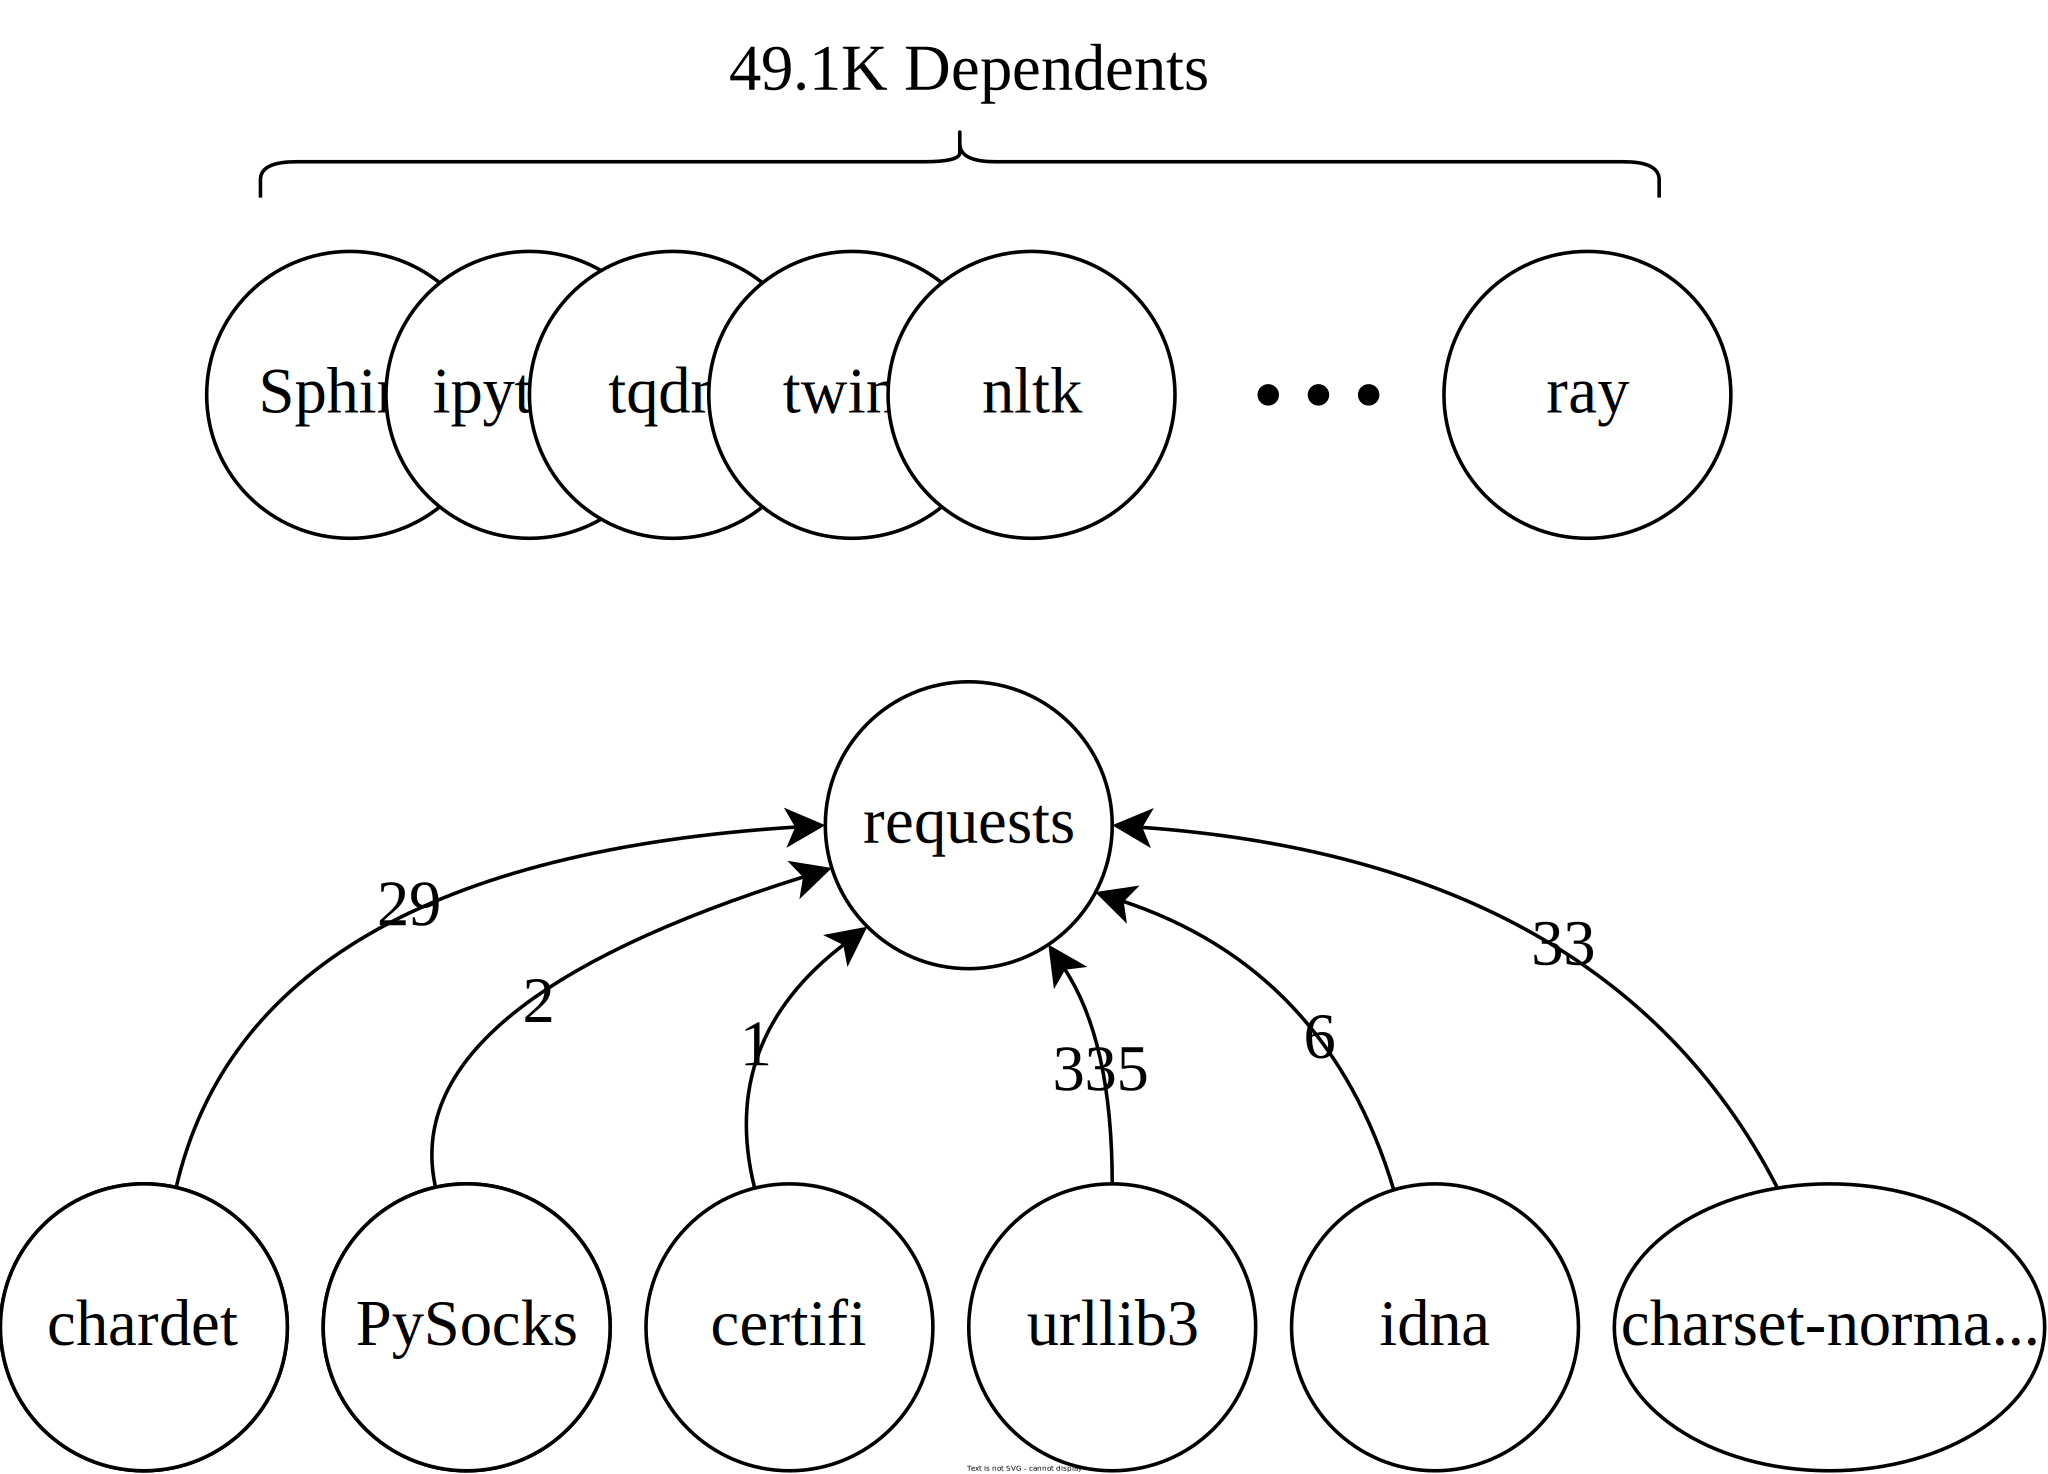
\includegraphics[width=0.8\linewidth]{figs/cs2.png}
  \caption{Dependency graph with API breaking change count as edge weights for the package \texttt{requests}}
  \label{fig6}
\end{minipage}\hfill
\end{figure}

\textbf{Analysis.} We observe that different packages pose different amounts of risk to other packages. One package poses more risk if it has more API changes or is being used by many other packages. Also, one could consider the indirect pose of risk through multiple nodes in this graph. 

\section{Discussion}
The goal of the case studies demonstrated in the previous section is not to conclude generalizable statements about the entire ecosystem of Python packages. We aim to show how a practitioner can use the underlying ideas and potentially the suggested implementation and apply them to their context. For instance, a library maintainer can create a dependency graph similar to what we depicted for their own package and even further extend it to more layers. It would also be possible to consider alternative dependencies and calculate the API breaking changes to help clients choose the less risky packages.

There are numerous possibilities for future researchers to extend different parts of our study. For instance, one paper could analyze the root cause of the increased dependency modification frequency in recent years. We manually analyzed some projects and observed that one reason could be the trend of using bots to keep the dependencies updated automatically. However, more empirical data is needed to get more generalizable insights.


\section{Threats to Validity}
\textbf{Construct Validity.}
In the first step of our study, we find \texttt{requirements.txt} files to identify the dependencies for each project. However, there are numerous other ways for a Python Project to manage its dependencies. It is even possible that projects use multiple methods for dependency management or change their method at some point in time. To completely resolve this issue, it would be necessary to consider all possibilities which are not practical and not that valuable for the goals that we had in mind. We focus on one of the most popular methods for Python dependency management to minimize the risk of not including all version changes. We also observe that for most projects, the frequency of version changes increases over time, which suggests that most projects probably do not switch their method of dependency management. Moreover, we discarded the projects with too few requirement changes.

\textbf{Internal Validity.}
In the second case study (the dependency graph), we suggest one form of interpretation: the graph weights can be seen as the amount of risk one node poses to another. One could object that, based on this interpretation, it would always mean that the package that has more weight on its edge to a node poses more risk on another package with a lower edge weight (i.e., fewer API breaking changes). One way to mitigate this issue would be to calculate a form of weighted average based on the severity offered by \texttt{AexPy}. However, in \cite{aexpy}, there is no clear explanation for their chosen severity level. In that case, there is the problem of subjectivity. Another way of mitigating this issue would be to statically analyze the client code base and count how many of those API breaking changes are among the API usage of the client. The problem with this idea is performance and lack of practicality. The end goal here is that future researchers could extend the concept of this case study to generate more extensive graphs based and help clients choose how they want to decide their dependencies more wisely. With that goal in mind, running static analysis to find API usage per client and pair of package dependencies would be impractical.  

\textbf{External Validity.} In the second part of RQ1, we narrowed our analysis to only 20 projects due to time constraints. This can limit the generalizability of the results based on the data extracted from the requirement modifications in those 20 projects. We acknowledge this as a potential shortcoming of our study and aim to mitigate this issue in future works.


\section{Conclusions}
We conduct the first empirical study on Python projects in the context of API breaking changes and dependency version changes. This study shows that most projects modify their dependencies every two months. Based on empirical results, we observe that projects follow different patterns of modifying the version of their dependencies over time. However, overall, most projects increase the frequency of their dependency version changes over time. We observe that non-major changes outnumber major changes (in terms of semantic versioning) by a far margin. Some packages tend to be updated or downgraded more than others. Through our first case study, we demonstrate how different types of API changes can occur in a single package. Our second case study shows how API breaking changes in a library can pose risks to its clients directly and indirectly. For future works, we aim to expand our analysis to cover more Python projects and find statistical relationships between their build failures and the API breaking changes of their dependencies. 
  

\bibliographystyle{IEEEtranN}
\bibliography{references}

\end{document}
